\subsection{Computer Vision and Landing Methodologies}
\label{sec:cv-and-landing}

Project: Icarus uses machine learning software running on the NVIDIA Jetson to
automatically and accurately identify landing pads. Once an appropriate pad is
selected, the aircraft begins the autonomous landing sequence.

\subsubsection{Landing Pad Recognition}

The UAS uses a global shutter camera to take clear and accurate images of the
ground. The image is ingested into the Yolov7 object detection model where
landing pad locations are extracted. As ground image is gathered, statistical
analysis is run until the confidence threshold is reached.

If no landing pad is initially found, the aircraft executes an overlapping
spiral search pattern, starting from the GPS coordinates of the waypoint. The
camera has a narrow field of view for greater detail so that detected pads are
not missed. If a landing pad still is not find in the designated search area,
the UAS switches into tele-operated control to land or reroute as required.

\begin{figure}[H]
        \centering
        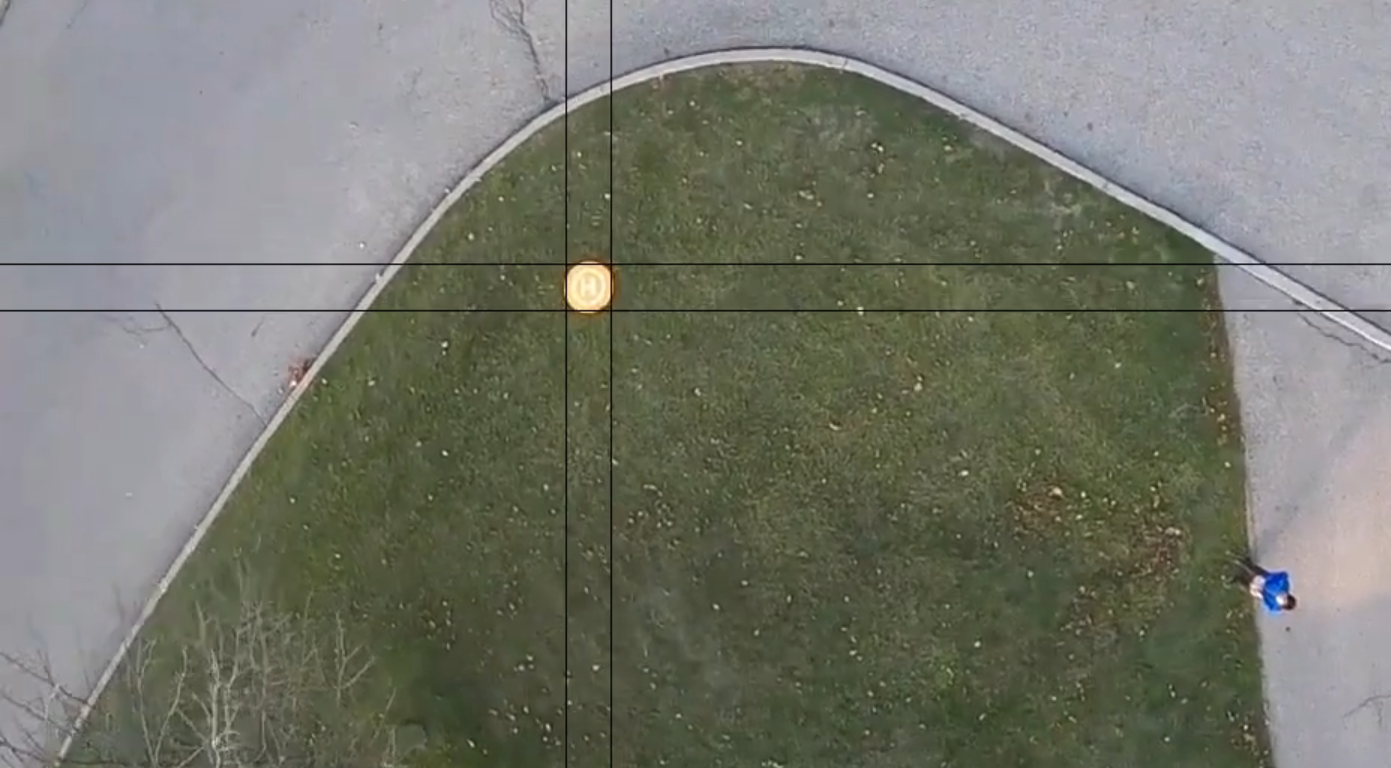
\includegraphics[width=\textwidth]{landing-pad}
		\caption{Landing pad detection algorithm overlayed over CV camera
		footage}
\end{figure}

\subsubsection{Autonomous Landing Sequence}
\label{sec:landing-sequence}

During the autonomous landing sequence, the aircraft hovers directly over the
selected landing pad. Images of the landing pad location are taken to confirm
the safety of the pad. Once this safety check is complete, the aircraft lands
automatically and passengers can safely disembark and embark the aircraft.
Otherwise, the UAS restarts the search pattern centred at the last known
landing pad location. If this is the second landing attempt, the UAS switches
to tele-operated control to land or reroute as required.

\subsubsection{ZeroPilot and NVIDIA Jetson Communication}
\label{sec:zp-jetson-communication}

The NVIDIA Jetson and ZeroPilot's PM submodule communicate during flight to
ensure the aircraft is accurately aligned with the landing pad. TM uses LOS'
UART driver to facilitate this communication. Messages from ZP to the Jetson
include telemetry and movement requests. Jetson to ZP messages include relative
movement commands for search execution and, when the aircraft confirms that it
is safe to land, a landing initiation request to PM.
